% 6. Results and Validations  
%   6.1. Anatomical Surrogate
%   6.2. Mechanical Simulation
\section{Results and Validations}
\label{sec:results_and_validations}

% - Disegno surrogato anatomico dell'albero respiratorio.  (output da
%   ParaView).
% - Grafici: un gradino "sopra" (10) le soglie e uno "sotto" (8) (xlims
%   = (.995, 1.09)).

% Grafici dipendenti dal numero di generazioni (?)

\subsection{Anatomical Surrogate}
\label{subsec:anatomical_results}

% Printscreen di ParaView colorcoded rispetto ai raggi.
Anatomy of the airway tree can be displayed by using ParaView.
\begin{figure}[H]\centering
  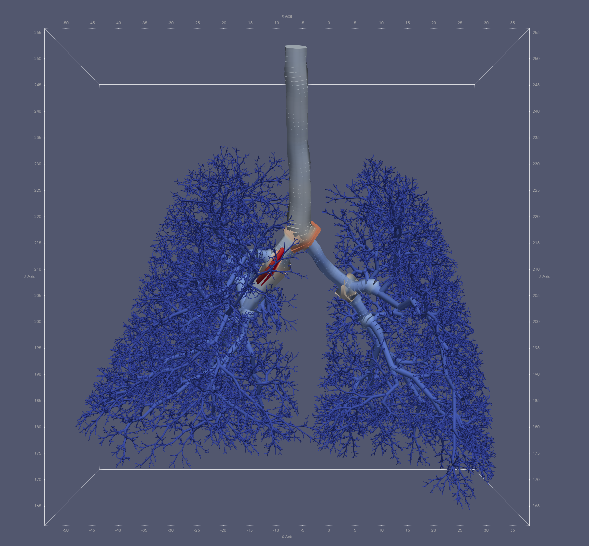
\includegraphics[scale=.6]{airways.png}
  \caption{3D rendered airway tree.}
  \label{fig:airways_results}
\end{figure}

\subsection{Mechanical Simulation}
\label{subsec:mechanical_results}

% Descrizione dei test.  La descrizione della rete in termini di
% parametri va fatta qui?

Different tests are displayed.  They consider as thresholds value
``vin\_th'' for each module diodes.

The first result describes modules voltages and currents, given a
over-threshold stimulation for all of them.

% Inserisco gli output di Julia, in particolare correnti e tensioni
% sotto e sopra threshold. (ampiezza scalino di 8 e 10V).

\begin{figure}[H]\centering
  \subfloat[][Airways voltages]{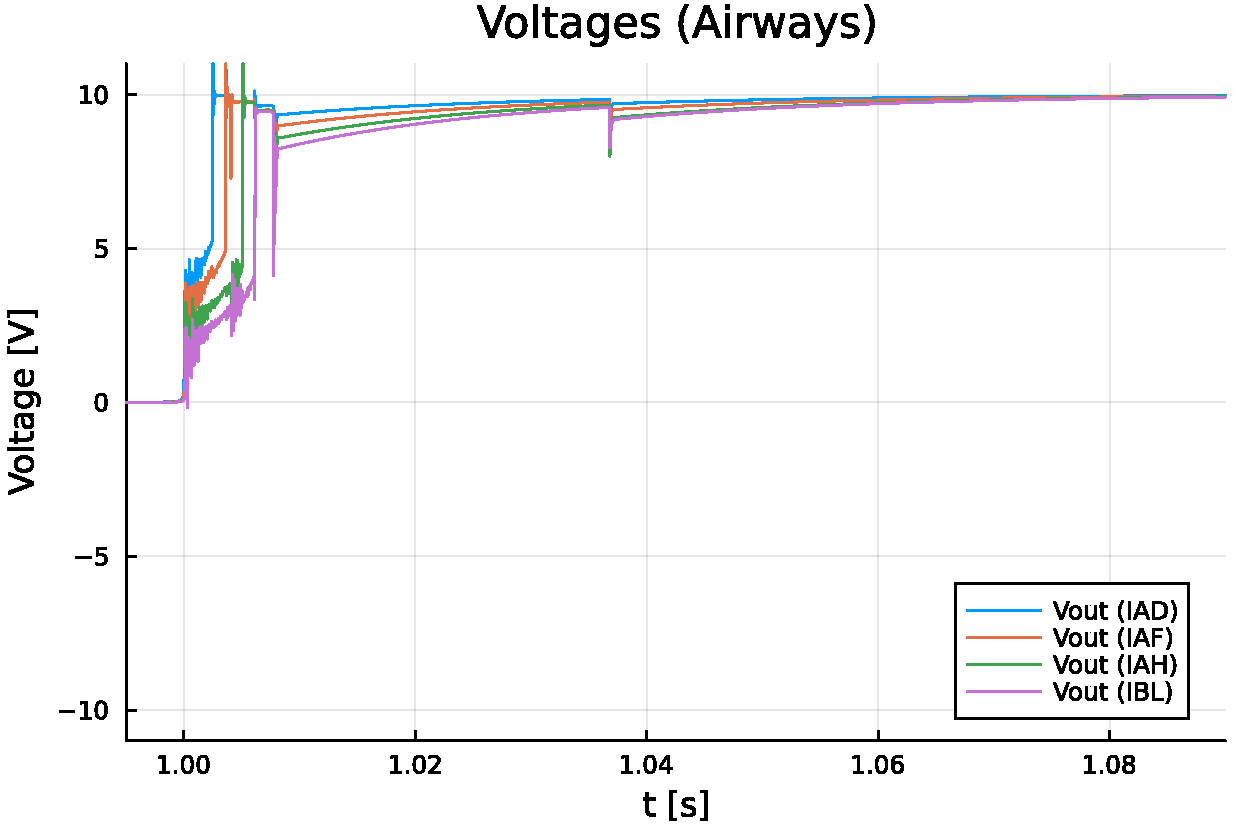
\includegraphics[height=.17\textheight]{airways_voltages_10.pdf}}  \subfloat[][Airways currents]{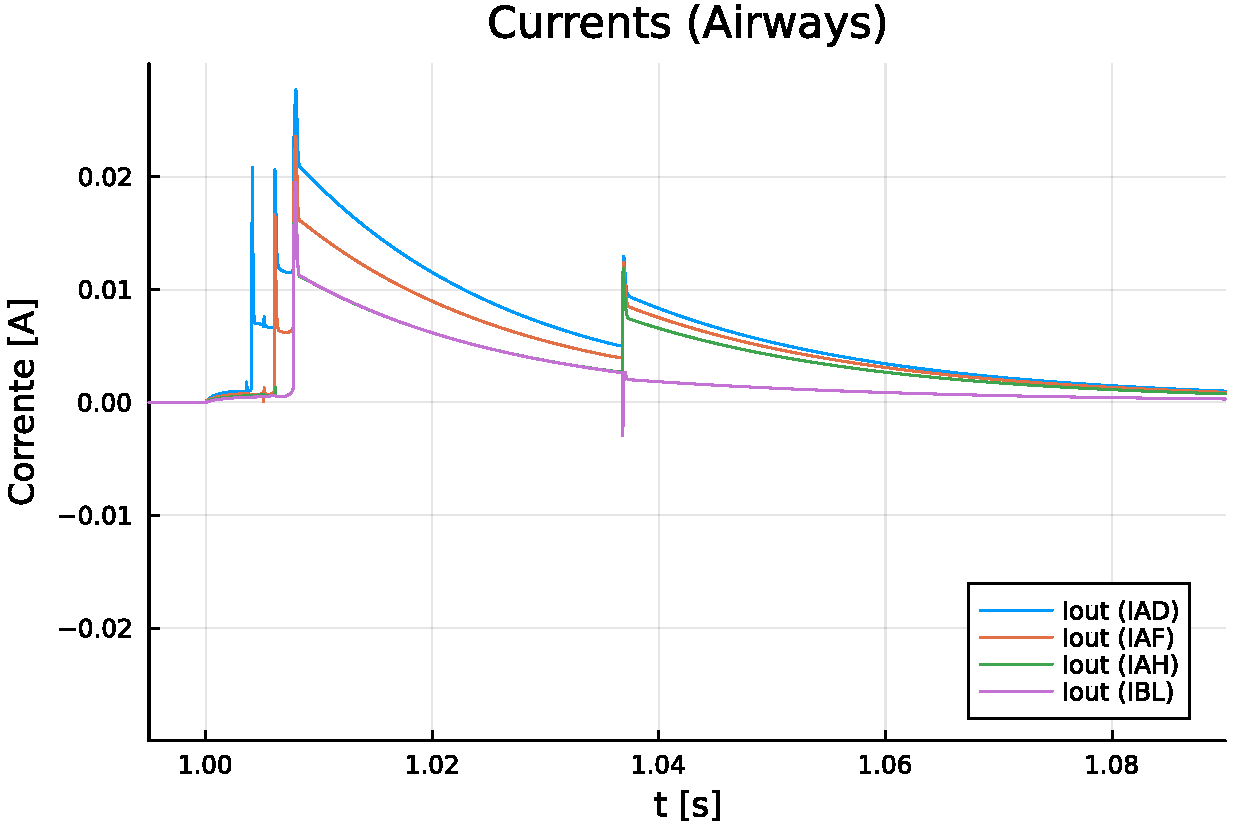
\includegraphics[height=.17\textheight]{airways_currents_10.pdf}}\\
  \subfloat[][Alveoli voltages]{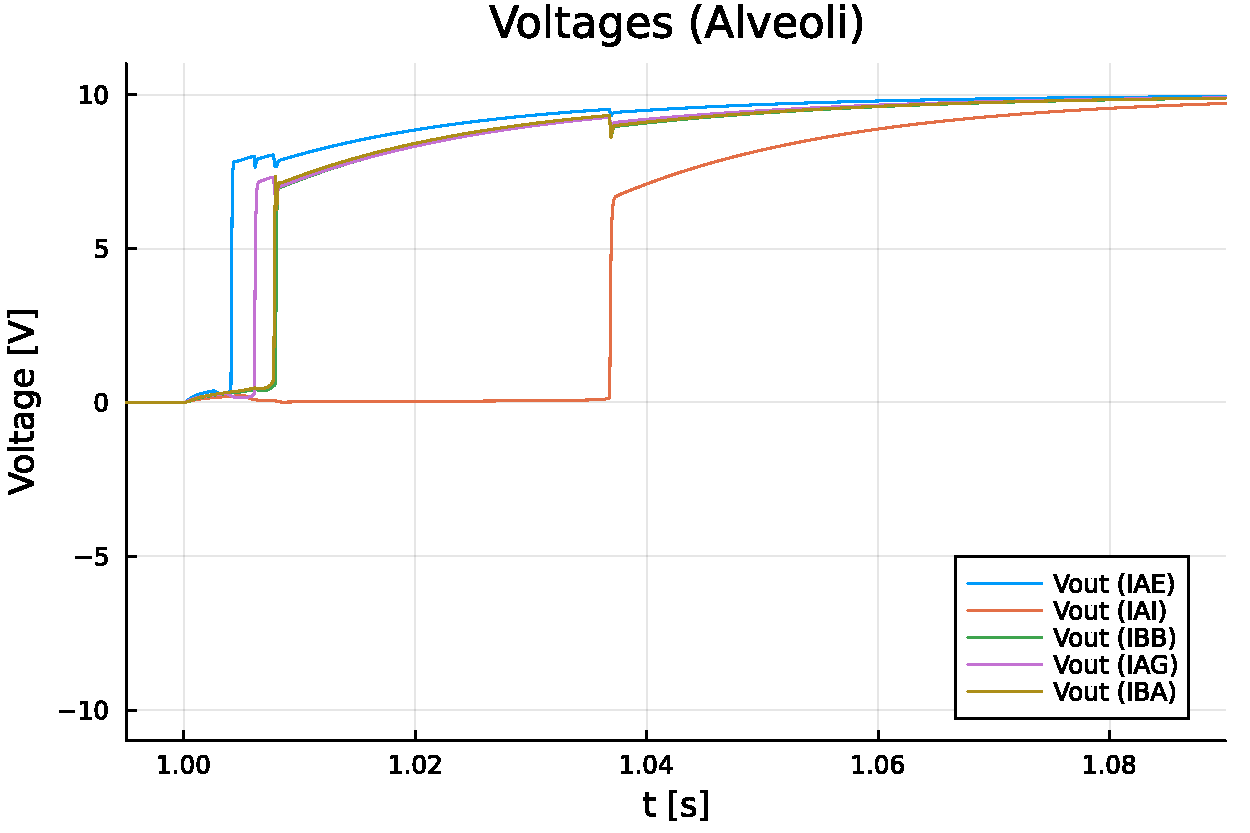
\includegraphics[height=.17\textheight]{alveoli_voltages_10.pdf}}  \subfloat[][Alveoli currents]{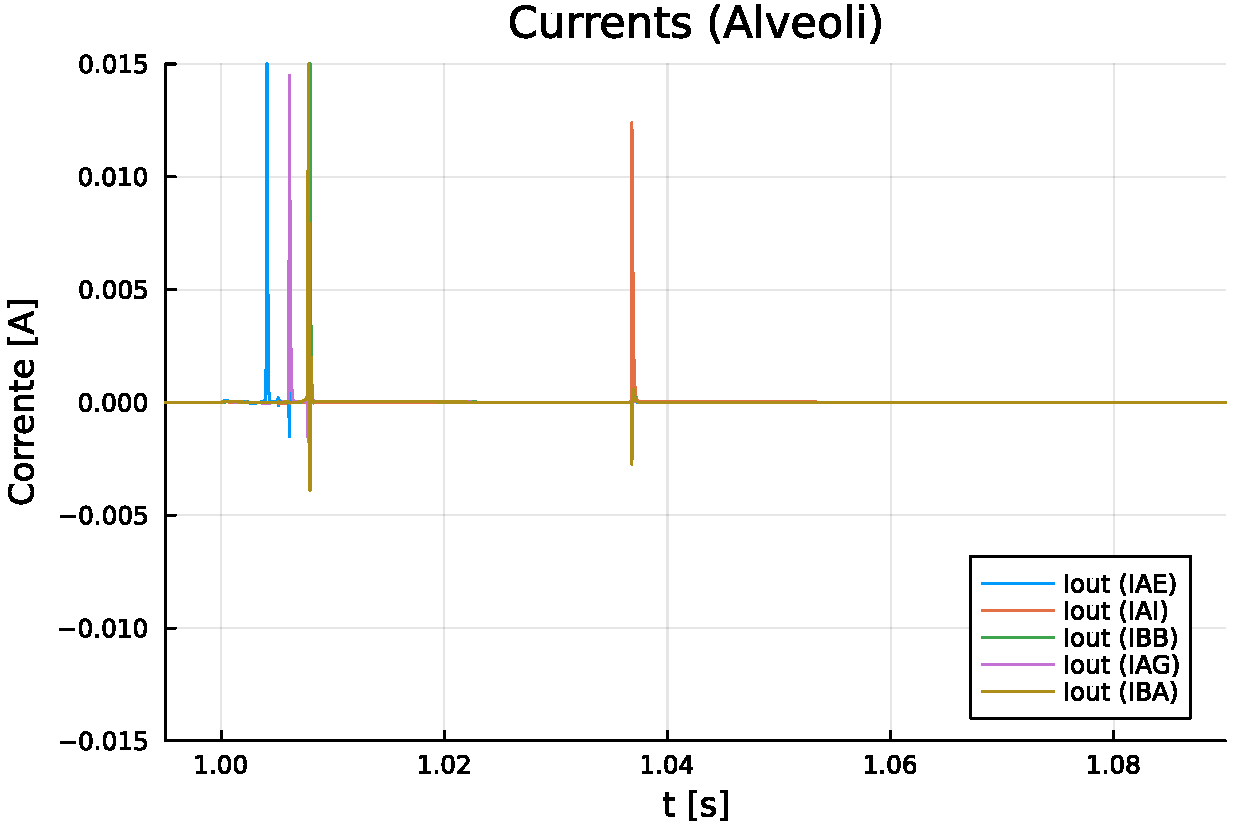
\includegraphics[height=.17\textheight]{alveoli_currents_10.pdf}}
  \caption{(Electrically equivalent) mechanical simulation for alveoli
    and aiways.  Step amplitude is 10V.}
  \label{fig:mechanical_results_above}
\end{figure}

The second one shows modules voltages and currents, given a
under-threshold stimulation for some alveoli (IAE, IAI and IAG).

\begin{figure}[H]\centering
  \subfloat[][Airways voltages]{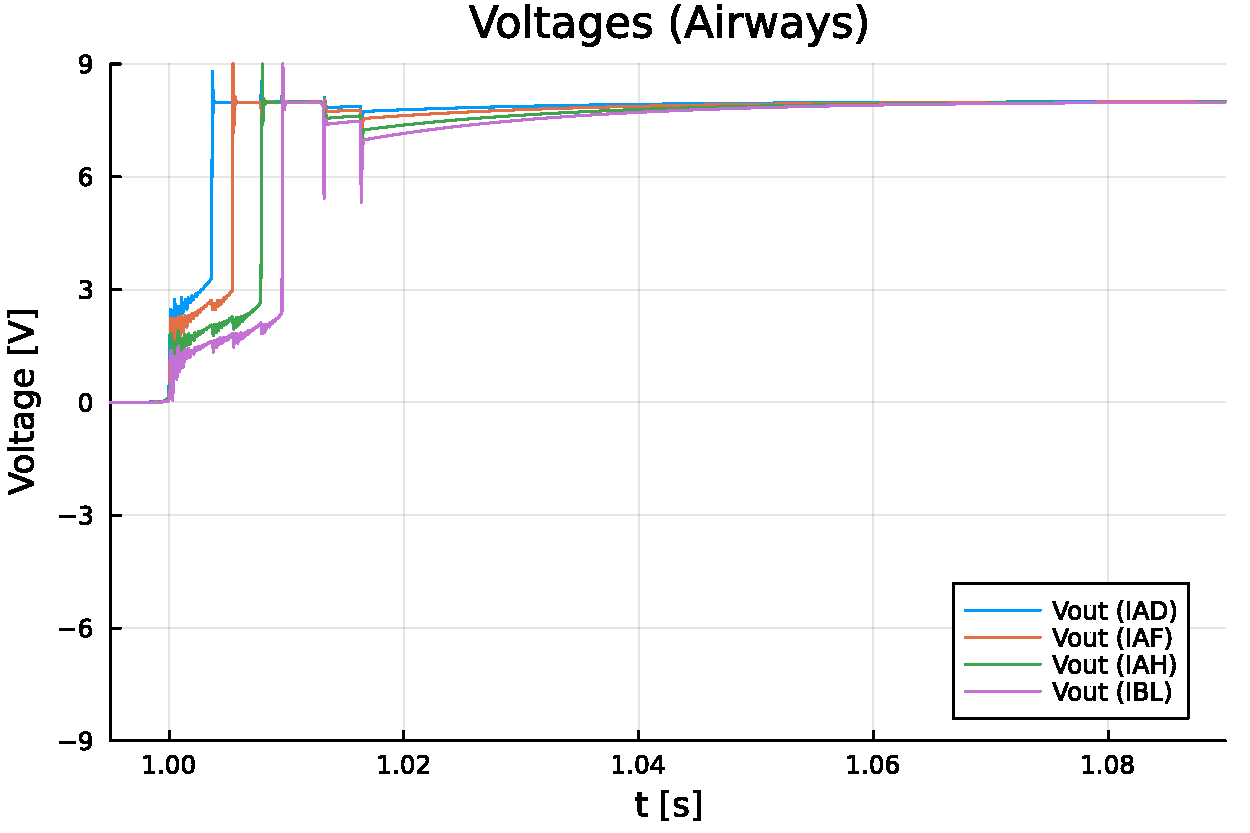
\includegraphics[height=.17\textheight]{airways_voltages_8.pdf}}  \subfloat[][Airways currents]{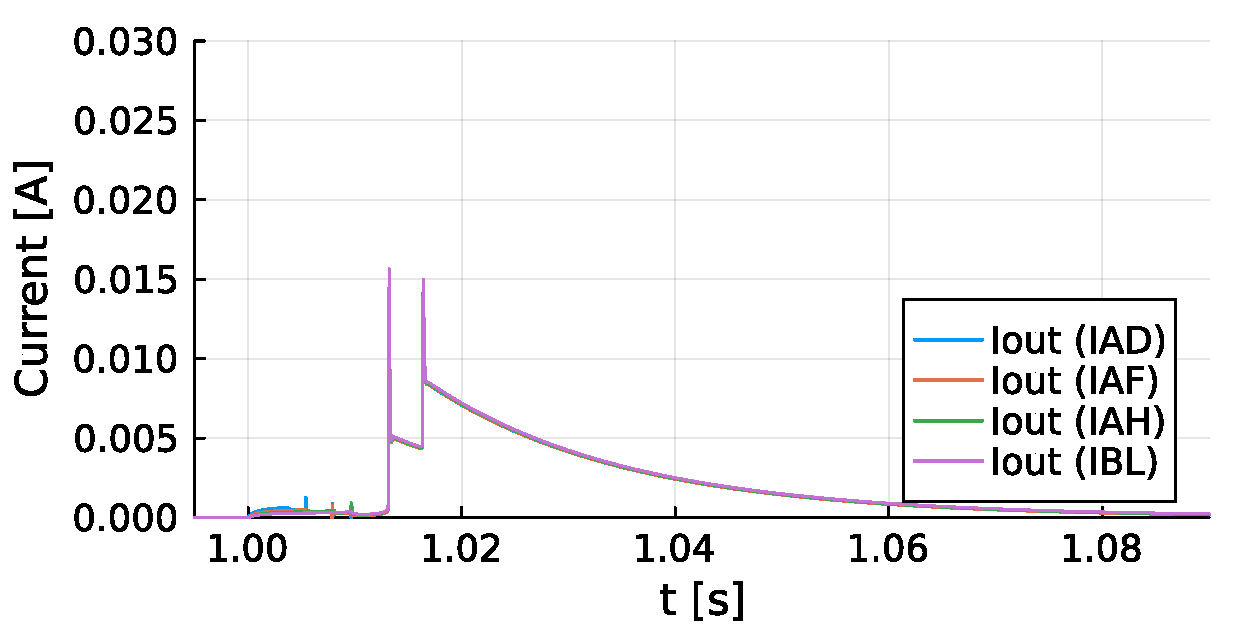
\includegraphics[height=.17\textheight]{airways_currents_8.pdf}}\\
  \subfloat[][Alveoli voltages]{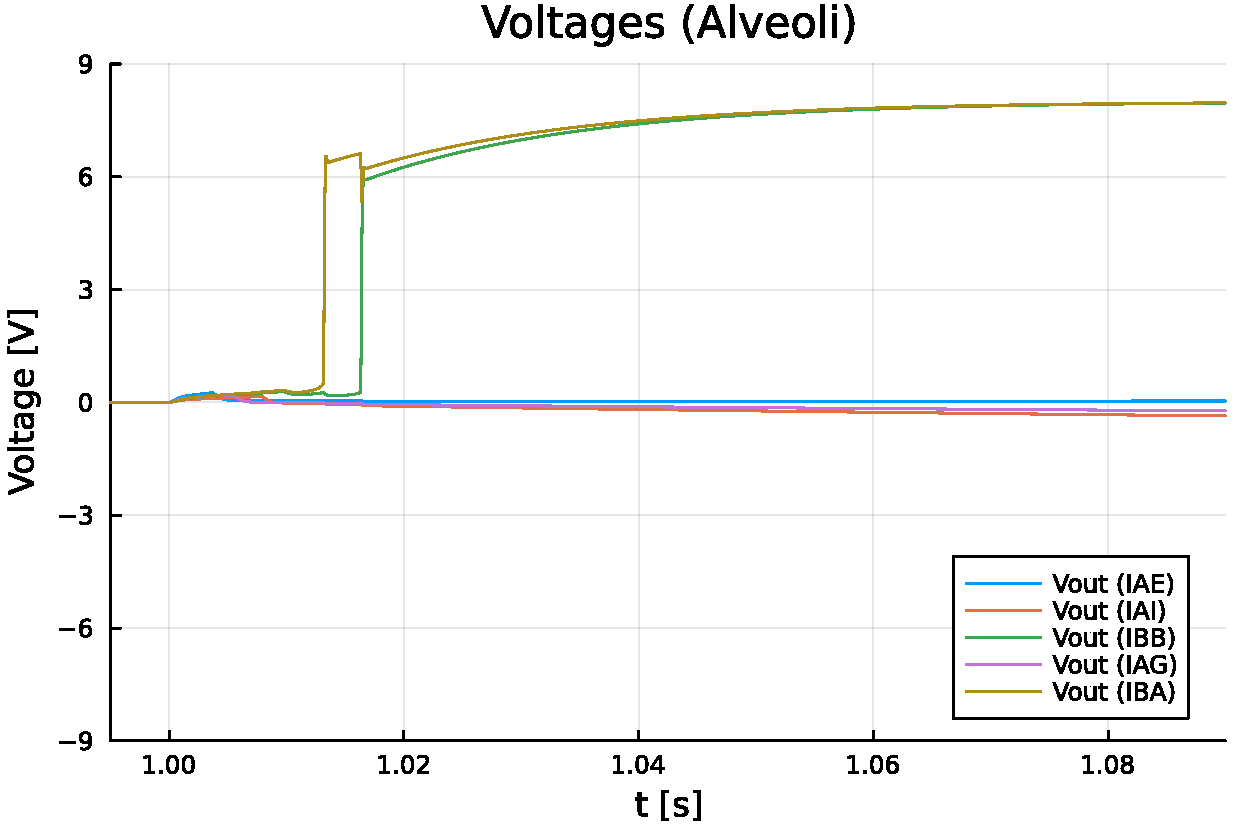
\includegraphics[height=.17\textheight]{alveoli_voltages_8.pdf}}  \subfloat[][Alveoli currents]{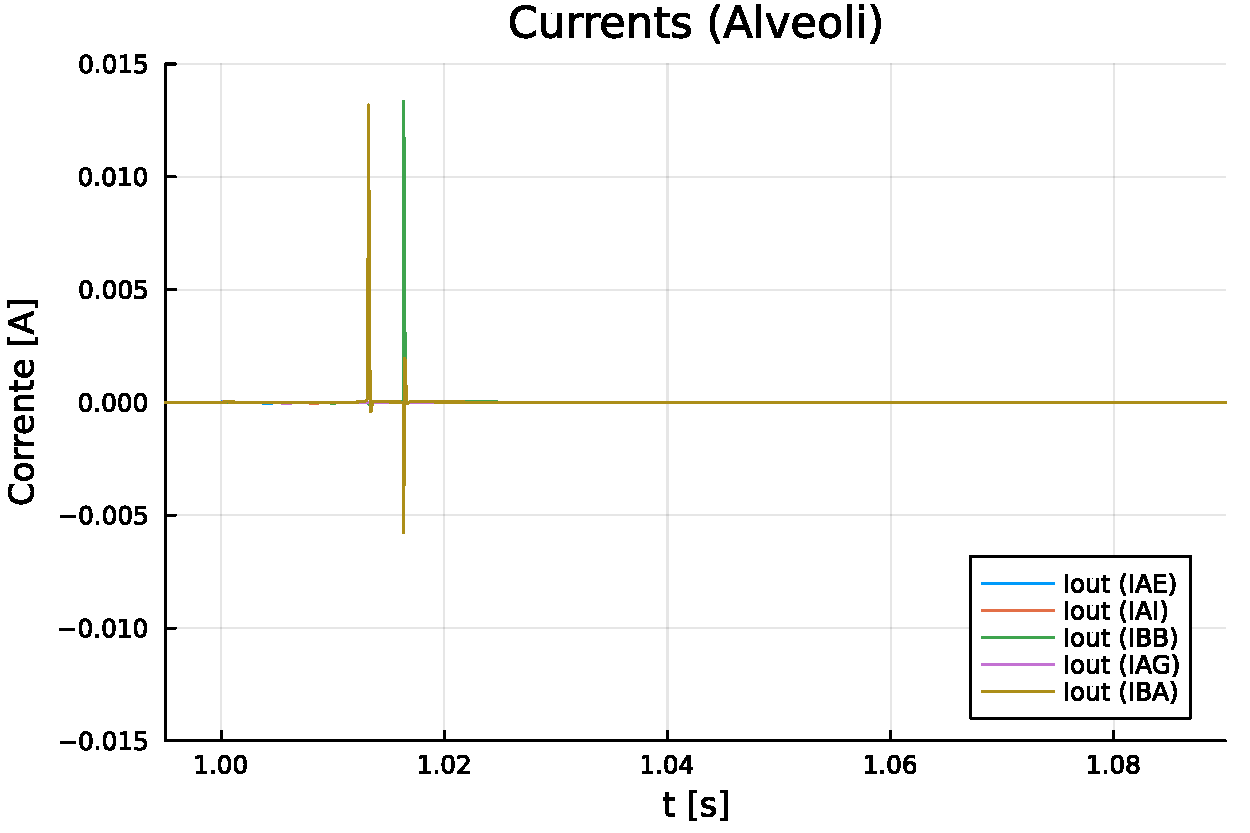
\includegraphics[height=.17\textheight]{alveoli_currents_8.pdf}}
  \caption{(Electrically equivalent) mechanical simulation for alveoli
    and aiways.  Step amplitude is 8V.}
  \label{fig:mechanical_results_below}
\end{figure}


%%% Local Variables:
%%% mode: LaTeX
%%% TeX-master: "../Thesis"
%%% End:
